\documentclass[aps,prl,twocolumn,superscriptaddress,showpacs,amsmath,amssymb]{revtex4-2}

% Packages
\usepackage[utf8]{inputenc}
\usepackage[T1]{fontenc}
\usepackage{textcomp}
\usepackage{mathtools, extarrows}
\usepackage[colorlinks,linkcolor=blue,citecolor=red,urlcolor=blue,bookmarks=true]{hyperref}
\usepackage{subcaption}
\usepackage{xcolor}
\usepackage{graphicx}% Include figure files
\usepackage{import}
\usepackage{xifthen}
\usepackage{transparent}
\usepackage{dcolumn}% Align table columns on decimal point
\usepackage{bm}% bold math
%\usepackage[mathlines]{lineno}% Enable numbering of text and display math
%\linenumbers\relax % Commence numbering lines

%\usepackage[showframe,%Uncomment any one of the following lines to test 
%%scale=0.7, marginratio={1:1, 2:3}, ignoreall,% default settings
%%text={7in,10in},centering,
%%margin=1.5in,
%%total={6.5in,8.75in}, top=1.2in, left=0.9in, includefoot,
%%height=10in,a5paper,hmargin={3cm,0.8in},
%]{geometry}


% PATHs
\graphicspath{{Figs/}}

\begin{document}

\title{Asymmetric second-order coherence function in atomic arrays}

\author{Nikita Nefedkin}
\affiliation{Photonics Initiative, Advanced Science Research Center, City University of New York, New York, NY 10031, USA}
\email{nnefedkin@gc.cuny.edu}

\author{Andrea Alù}
\affiliation{Photonics Initiative, Advanced Science Research Center, City University of New York, New York, NY 10031, USA}
\affiliation{Physics Program, Graduate Center, City University of New York, New York, NY 10016, USA}
\email{aalu@gc.cuny.edu}

% Keywords section is not typical in revtex; however, you can include it as follows:
\keywords{Quantum nonreciprocity, Subradiance, Dark state, Quantum isolator}

\begin{abstract}
    We study the second-order coherent function in the array of two-level atoms. 
    Under the conditions of geometric asymmetry or the detuning of one or more atoms in the array, we predict the incident wave direction dependent $g^{(2)}(0)$. 
    Moreover, at the optimal parameters of the array, the emission statistics may demonstrate bunching and antibunching dependence with respect to the direction of the incident excitation.
\end{abstract}

\maketitle

\section{Introduction}\label{sec:intro}

Transition from unitary quantum objects to complex many-body systems allowing macroscopic quantum states. 
The importance of utilizing collective behaviour of many-body systems in collective states and new horizons in quantum information processing.
Relation to superradiance~\cite{nefedkin2016superradiance} and subradiance.
Importance of controlling the statistical properties of emission from atomic systems in real applications.
Utilizing nonreciprocity in the context of emission statistics, however, this cannot be called nonreciprocity directly -- the term asymmetry fits better.

In this work, we study the emission from arrays of two-level atoms depending on the direction of the incident EM wave.
We focus mostly on the emission statistics and way to control and distinguish the collective and individual emission.

\section{Atomic chain interacting with the incident EM wave}

We start from the general consideration of a system of atoms aligned in a chain. 
Let us consider $N$ two-level atoms located along $z$ axis with a period $a$.
For simplicity, we assume that all atoms have the same dipole moment $\mathbf{d} = d \mathbf{e}_x$, oriented along $x$.
We denote $|g_j\rangle$ and $|e_j\rangle$ the ground and excited states of the $j$th atom, $j = 1, \ldots, N$.
The transition rate between these states we denote as $\omega_j$.
Each atom, considered single in free space, spontaneously emits with rate $\gamma_0^j = \frac{\omega_j^3 d^2}{3 \pi \epsilon_0 \hbar c^3}$~\cite{carmichael1999statistical}, where $\epsilon_0$ is the vacuum permittivity and $c$ is the speed of light.
In the following, for simplifying the notation, we normalize the decay rates of atomic collective modes by the spontaneous emission rate of a single atom in free space.

To excite the atom chain, we consider a monochromatic electromagnetic (EM) plane waves.
For simplicity, we consider these waves to propagate along the $z$ axis, i.e. along the array of atoms.
Of course, it is straightforward to generalize the consideration to tilted excitation directions.
The incident electric field is $\mathbf{E}_\mathrm{in}(\mathbf{r})e^{- i \omega_0 t} = E_0 \mathbf{e}_x e^{i \mathbf{k}_0 \mathbf{r}} e^{- i \omega_0 t}$, where the wave vector $\mathbf{k}_0 = \pm k_0 \mathbf{e}_z$ has absolute value $k_0$ and points towards either the $+z$ or $-z$ direction. For
brevity, we define as \textit{forward} $+z$ direction and as \textit{backward} $-z$ direction, see Fig.~\ref{fig:01}.

\begin{figure}[h]
    \centering
    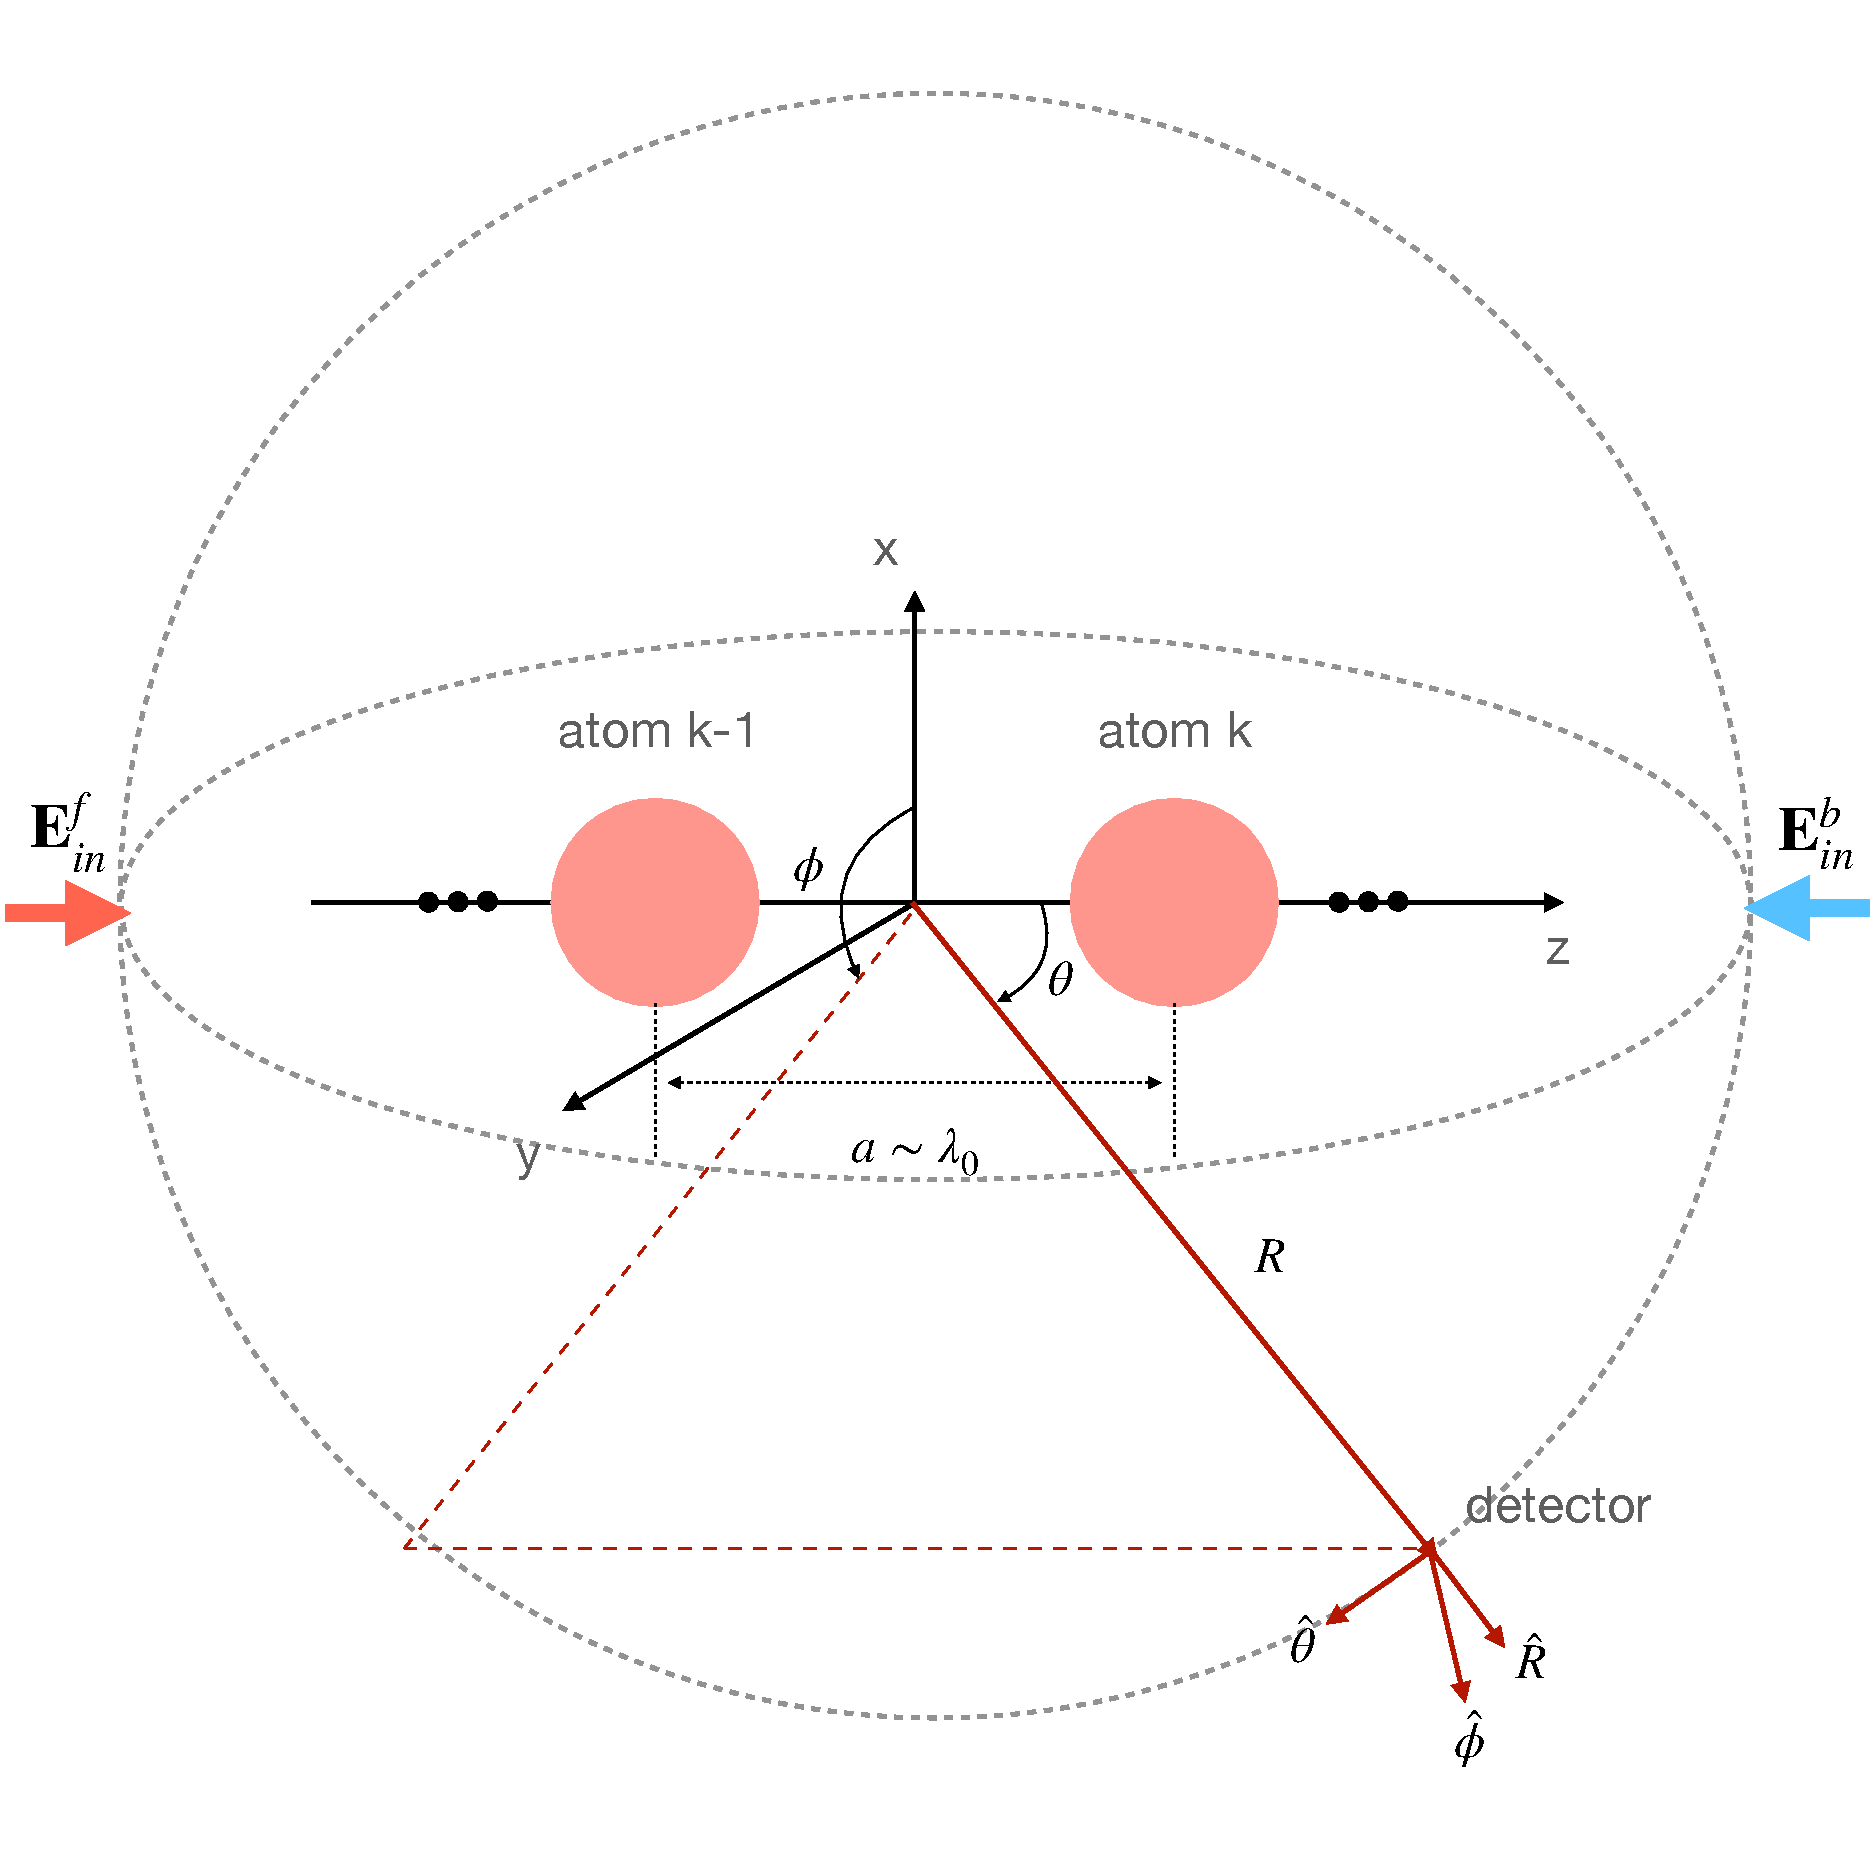
\includegraphics[width=0.9\linewidth]{fig1_sketch}
    \caption{Chain of two-level atoms interacting with incident EM waves propagating in $+z$ ($f$) direction and $-z$ ($b$) direction. The emission from the array is registered by detectors in the far field zone, the positions of the detectors are written in spherical coordinates.}
    \label{fig:01}
\end{figure}

The full description of the system depicted in Fig.~\ref{fig:01} includes taking into account the continuum of EM modes of free space and all the degrees of freedom of the atoms, as well as the interaction between the EM modes and atoms. 
This approach turns out to be challenging to even find an approximate numeric solution, therefore, we follow the standard procedure \cite{carmichael1999statistical,bettles_quantum_2020,wild_algorithms_nodate} of eliminating the field degrees of freedom considering them as a thermal reservoir with the temperature close to zero.
This is possible by applying the Born-Markov approximation. 
Assuming that the relaxation time of the atoms is much slower than the relaxation time of the photonic reservoir and the time required by light to propagate between atoms, the photonic degrees of freedom can be traced out from the full Hamiltonian of the system, resulting into an effective master
equation which involves only atomic degrees of freedom.
Quantitatively, the Born-Markov approximation requires the $\gamma_{\mathrm{max}}^{-1} \gg a_\mathrm{max} / c$, where $\gamma_\mathrm{max}$ is the largest atomic decay rate, and $a_\mathrm{max}$ is the largest inter-atomic distance in the array.
The effective master equation reads as follows:
\begin{align} \label{eq:01}
    \dot{\hat{\rho}} =& \frac{i}{\hbar}\left[ \hat{\rho}, \hat{H}_S \right] + \nonumber \\
                      & \sum_{i,j=1}^N \frac{\Gamma_{ij}}{2}\left( 2 \hat{\sigma}_j \hat{\rho} \hat{\sigma}^+_i - \hat{\rho} \hat{\sigma}^+_i \hat{\sigma}_j - \hat{\sigma}^+_i \hat{\sigma}_j \hat{\rho}\right).
\end{align}
Here the lowering and raising operators $\hat{\sigma}_j = \underbrace{\hat{I} \otimes \ldots \otimes}_{j-1} \hat{\sigma}_j \underbrace{\otimes \ldots \otimes \hat{I}}_{N-j} $ and $\hat{\sigma}_j^+ = \underbrace{\hat{I} \otimes \ldots \otimes}_{j-1} \hat{\sigma}_j^+ \underbrace{\otimes \ldots \otimes
\hat{I}}_{N-j}$ describe the relaxation and excitation of the $j$th atom, where $\hat{\sigma} = |g\rangle \langle e|$ and $\hat{\sigma}^+ = |e\rangle \langle g|$ are transition operators between excited $|e\rangle$ and ground $|g\rangle$ states; $\hat{I}$ is the identity operator.
Note that here we assumed that the thermal excitations in the reservoir are negligible due to the close to zero temperature of the reservoir, and thus dissipation takes place only from the atomic system to the reservoir and not vise versa.
For an ensemble of atoms arbitrary arranged with regard of restrictions of the Born-Markov approximation, the effective Hamiltonian of the system in the rotating frame with the frequency of the incident EM field $\omega_0$ is \cite{bettles_quantum_2020,asenjo-garcia_exponential_2017,shahmoon_cooperative_2017}
\begin{align} \label{eq:02}
    \hat{H}_S =& \hbar \sum_{k=1}^N \left( \frac{\Delta_k}{2} \hat{\sigma}_z^k - \Omega_R^k \hat{\sigma}_k - \Omega_R^{k*} \hat{\sigma}_k^+ \right) + \nonumber \\
               & \hbar \sum_{i \neq j}^N \Omega_{ij} \hat{\sigma}_i^+ \hat{\sigma}_j,
\end{align}
where the indices $k,i,j$ run over all the atoms and $\hat{\sigma}_z^k = \left[ \hat{\sigma}_k^+, \hat{\sigma}_k \right]$ stands for the population inversion of the $k$th atom. 
The detuning between the $k$th atom and the incident field we define as $\Delta_k = \omega_k - \omega_0$, and the interaction constant between the incident field and the $k$th atom, $\Omega_R^k = \mathbf{d} \cdot \mathbf{E}_\mathrm{in}^+ (\mathbf{r}_k) / \hbar$. 
For a fixed dipole moment of the atomic transition and the fixed position of the atom, the interaction constant is proportional to the incident field amplitude in the coordinate of the atom. 
The effective dipole-dipole interaction arises in the system due to interaction of the atoms with the EM modes of free space. 
The constant of the dipole-dipole interaction between $j$th and $k$th atoms takes the form:
\begin{align} \label{eq:03}
    \mathcal{H}_{jk} &= - \frac{3 \pi c}{\omega} \sqrt{\gamma_0^j \gamma_0^k} \mathbf{d}_j^* \bar{\bar{\mathbf{G}}}(\mathbf{r}_j, \mathbf{r}_k, \omega) \mathbf{d}_k  \\
                     & = \Omega_{jk} - \frac{i}{2} \Gamma_{jk} \nonumber
\end{align}
where the real part is responsible for coherent interactions and the imaginary part -- for dissipative interactions.
In eq.~(\ref{eq:03}), $\bar{\bar{\mathbf{G}}}$ is the free-space Green's tensor that reads
\begin{equation}
    \bar{\bar{\mathbf{G}}}(\mathbf{r}, \mathbf{r}', k) = \left[ \bar{\bar{\mathbf{I}}} + \frac{1}{k^2} \nabla \nabla \right] \frac{e^{i k |\mathbf{r} - \mathbf{r}'|}}{4 \pi |\mathbf{r} - \mathbf{r}'|}
    \label{eq:04}
\end{equation}
and $\bar{\bar{\mathbf{I}}}$ is a unit tensor of the second order.

In this work, we focus on the statistical properties of the atomic array. 
The key characteristic reflecting the statistical nature of the emission from the array is the second-order coherence function defined as follows \cite{mandel1995optical}:
\begin{align}
    & g^{(2)}(\mathbf{R}_1, t_1; \mathbf{R}_2, t_2) = \nonumber \\ 
    & \frac{\langle \hat{\mathbf{E}}_\mathrm{sc}^{(-)} (\mathbf{R}_1, t_1) \hat{\mathbf{E}}_\mathrm{sc}^{(-)} (\mathbf{R}_2, t_2) \hat{\mathbf{E}}_\mathrm{sc}^{(+)} (\mathbf{R}_2, t_2) \hat{\mathbf{E}}_\mathrm{sc}^{(+)} (\mathbf{R}_1, t_1)\rangle}{\langle
    \hat{\mathbf{E}}_\mathrm{sc}^{(-)} (\mathbf{R}_1, t_1) \hat{\mathbf{E}}_\mathrm{sc}^{(+)} (\mathbf{R}_1, t_1) \rangle \langle \hat{\mathbf{E}}_\mathrm{sc}^{(-)} (\mathbf{R}_2, t_2) \hat{\mathbf{E}}_\mathrm{sc}^{(+)} (\mathbf{R}_2, t_2) \rangle} 
    \label{eq:05}
\end{align}
This is the $g^{(2)}$ function for the field scattered from the atom array, which operator is given by:
\begin{equation} 
    \hat{\mathbf{E}}_\mathrm{sc}^+(\mathbf{r}) = \frac{\omega^2}{\epsilon_0 c^2} \sum_{j=1}^N \bar{\bar{\mathbf{G}}}(\mathbf{r}, \mathbf{r}_j, \omega) \mathbf{d}_j \hat{\sigma}_j
    \label{eq:06}
\end{equation}

We will consider the way of calculating the second-order coherence function, eq.~(\ref{eq:05}), in the further sections in detail.

\section{Collective states in the ensemble of atoms}

\uppercase{Add good link and connection to the previous sections and give an explanation why we need to look at the collective behaviour of the system, give examples of nonreciprocity and asymmetric g2}

The many-body system consisting of $N$ atoms allows for the existence of the collective states which significantly modify its dynamics. 
Examples of these collective states are subradiant (or dark) state and superradiant (or bright) state.
The subradiant state is characterized with the slower decay rate then the decay rate of the individual atom in the array and has the form of fully antisymmetric state with regard to atoms' permutations~\cite{gross1982superradiance}.
In the case of an ensemble of atoms located in a subwavelength volume, the decay rate from the subradiant state is equal to zero.
The superradiant state, on the other hand, is the state with the fastest decay rate, proportional to $N^2$ if the atoms located in the subwavelength volume, and it has the form of fully symmetric state with regard to permutations of the atoms~\cite{gross1982superradiance}. 

For the system depicted in Fig.~\ref{fig:01}, the subradiant and superradiant states may be obtained by diagonalizing the effective non-Hermitian Hamiltonian:
\begin{equation} 
    \hat{H}_\mathrm{eff} = \hat{H}_S - i \hbar \sum_{j,k} \frac{\Gamma_{jk}}{2} \hat{\sigma}_j^+ \hat{\sigma}_k
    \label{eq:07}
\end{equation}
where the imaginary part accounts for dissipation.
However, in the general case, where $\omega_j \neq \omega_k$ and consequently $\gamma_0^j \neq \gamma_0^k$, $k \neq j$, $k,j = 1,\ldots, N$, it is difficult to diagonalize the Hamiltonian in eq.~(\ref{eq:07}).
Thus, to demonstrate the existence of the dark, $|D\rangle$, and bright, $|B\rangle$, states, we consider the system of two identical atoms in resonance with the incident field, $\omega_1 = \omega_2 = \omega_0$.
In this case, we can find the dark and bright states by diagonalizing only the dissipative part of the Hamiltonian (\ref{eq:07}), which is equivalent of diagonalizing the matrix $\left( \Gamma_{jk} \right)$~\cite{gross1982superradiance,carmichael2000quantum,clemens2003collective}.
Its eigenvalues gives the decay rates of the collective states in the system, namely, $|D\rangle$ and $|B\rangle$.
To obtain the form of these states, one needs to act by a corresponding collective operator on the ground state of the system, $|G\rangle$~\cite{carmichael2000quantum,clemens2003collective}.

In more general case of $N$ atoms, this procedure can be formalised in the following way. 
The collective operators or the source-mode jump operators have the form:
\begin{align}
    \vec{J} &= \sqrt{\Lambda} \mathbf{B} \vec{\Sigma} \label{eq:08a} \\
    \vec{J}^\dagger &= \vec{\Sigma}^\dagger \mathbf{B}^T \sqrt{\Lambda},
    \label{eq:08b}
\end{align}
where 
\begin{align}
    \left(\Gamma_{jk}\right) &= \mathbf{B}^T \Lambda \mathbf{B}, \;\; 
    \Lambda = \mathrm{diag}\left(\lambda_1, \ldots, \lambda_N \right) \\ 
    \vec{\Sigma} &= \left( \hat{\sigma}_1, \ldots, \hat{\sigma}_N \right)
    \label{eq:09}
\end{align}
The dissipative part of the master equation (\ref{eq:01}) rewrites in terms of collective operators (\ref{eq:08a}), (\ref{eq:08b}) as follows:
\begin{equation}
    \mathcal{D}_J(\cdot) = \frac{1}{2} \sum_{m=1}^N \left( 2 \hat{J}_m \cdot \hat{J}_m^\dagger - \hat{J}_m^\dagger \hat{J}_m \cdot - \cdot \hat{J}_m^\dagger \hat{J}_m \right),
    \label{eq:10}
\end{equation}
where operators $\hat{J}_m$ are collective operators, which are the elements of the vector (\ref{eq:08a}).

In the case of two atoms in the array, the dark and bright states decay rates are $\gamma_{B} = \gamma_0 + \Gamma_{12}$ and $\gamma_{D} = \gamma_0 - \Gamma_{12}$. 
Here we used the assumption of identical atoms, so $\Gamma_{11} = \Gamma_{22} = \gamma_0$. 
If we substitute $\Gamma_{12}$ using formula (\ref{eq:03}), we obtain the following expression for the decay rates of $|D\rangle$ and $|B \rangle$:
\begin{equation}
\frac{\gamma_{D/B}}{\gamma_0} = 1 \mp \frac{3 \left| k_0 a \cos \left( k_0 a \right)+ \left(k_0^2 a^2 -1\right)\sin \left( k_0 a \right)\right| }{2 k_0^3 a^3}
    \label{eq:11}
\end{equation}
where $k_0 = \omega_0 / c$.
Note that $\gamma_B = 2 \gamma_0$ and $\gamma_D = 0$ in the case of a subwavelength array, $a \to 0$, and these decay rates respond to the decay rates of conventional superradiant and subradiant states~\cite{dicke1954coherence,nefedkin2017bad,nefedkin2017superradiance}.
By applying the collective operators corresponding to $|D\rangle$ and $|B \rangle$ states to the ground state, we obtain these states in the uncoupled basis:
\begin{align}
    |D \rangle &= \frac{1}{\sqrt{2}} \left( |e,g\rangle - |g,e\rangle \right)\\
    |B \rangle &= \frac{1}{\sqrt{2}} \left( |e,g\rangle + |g,e\rangle \right)
\end{align}

As shown before~\cite{muller2017nonreciprocal,hamann2018nonreciprocity, nefedkin2022dark, nefedkin2023nonreciprocal}, the collective states play the pivotal role in nonreciprocity effects in many-body systems. 
By excitation of the system with an EM wave from one direction, the dark collective state becomes populated, whereas by excitation from the other direction, the system remains in the ground state. 
This asymmetry in system's state populations leads to nonreciprocal behaviour of the light scattered by the system. 
In this work, we utilize the idea of asymmetric system population to explore the statistical properties of the emission.

\section{Second-order coherence function for directed-detection operators}

Let us take a look at the expression for the second-order coherence function $g^{(2)}$, eq.~(\ref{eq:05}).
This expression defines the degree of coherence of the field scattered from the atomic array in two different points in space and time.
Physically, it is interpereted as two detectors located in points $\mathbf{R}_1$ and $\mathbf{R}_2$ measuring the signal from the array at times $t_1$ and $t_2$.

The expression (\ref{eq:06}) involves the operators of the scattered field, eq.~(\ref{eq:06}). 
These operators contain the sum over all atoms in the arrays and depend explicitly on the dyadic Green tensor of the environment.
In this form, it may be challenging to compute the correlation functions in the formula for the $g^{(2)}$ function.
Therefore, we restrist ourselves with the far-field approximation, e.g. the detectors are located much farther from the array then the wavelenght of the scattered field and the geometrical size of the array, $|\mathbf{R}_j| \gg \lambda_0, N a$, where $j$ is the index of the detector.

To take into account the photon emitted in the certain direction $\bar{\mathbf{R}}(\theta, \varphi) = \mathbf{R} / R$, where $\mathbf{R}$ is the coordinate of the detector and $R = |\mathbf{R}|$ (see Fig.~\ref{fig:01}), and detected within the element of solid angle $d \Omega$ in far field, we following
Ref.~\cite{carmichael2000quantum} introduce the direct detection operators:
\begin{equation}
    \hat{S}(\theta, \varphi) = \sqrt{\frac{2 \epsilon_0 c}{\hbar \omega_0} \left( R^2 d \Omega \right)} \hat{E}_\mathrm{sc}^+ (\mathbf{R}(\theta, \varphi), t),
    \label{eq:12}
\end{equation}
where the module of the operator of the scattered field in the far field takes the form:
\begin{align}
    \label{eq:13}
    &\hat{E}_\mathrm{sc}^+ (\mathbf{r}, t) = \frac{3 \hbar \gamma_0}{4 d k_0} \frac{\sqrt{1 - \left( \bar{\mathbf{d}} \cdot \bar{\mathbf{r}}^2 \right)}}{|\mathbf{r}|} \sum_{j=1}^N e^{-i k_0 \bar{\mathbf{r}} \cdot \mathbf{r}_j} \hat{\sigma}_j(t), \\
    & \bar{\mathbf{d}} = \frac{\mathbf{d}}{d}, \;\; \bar{\mathbf{r}} = \frac{\mathbf{r}}{|\mathbf{r}|} \nonumber
\end{align}
and $\mathbf{r}_j$ is the coordinate of the $j$th atom.
Substituting eq.~(\ref{eq:13}) in eq.~(\ref{eq:12}) and moving to spherical coordinates, we obtain the short form of the directed-detection operator:
\begin{equation}
    \hat{S}(\theta, \varphi) = \sqrt{\gamma_0 D(\theta, \varphi) d \Omega} \sum_{j=1}^N e^{-i k_0 \bar{\mathbf{r}}(\theta, \varphi) \cdot \mathbf{r}_j} \hat{\sigma}_j,
    \label{eq:14}
\end{equation}
where 
\begin{equation}
    D(\theta, \varphi) = \frac{3}{8 \pi} \left[ 1 - \left( \bar{\mathbf{d}} \cdot \bar{\mathbf{r}}(\theta, \varphi) \right)^2 \right]
    \label{eq:15}
\end{equation}
is the dipole radiation pattern for emission from an individual atom.
Note that the dissipative part of the master equation~(\ref{eq:01}) can be rewritten in terms of directed-detection operators (\ref{eq:14}), which have a clear physical interpretation of detecting scattered photons by the array of atoms in the direction $(\theta, \varphi)$.
Thus, the dissipative part takes the following form:
\begin{align}
    \label{eq:16}
    \mathcal{D}_S(\cdot) = \frac{1}{2} \int d \Omega & \left( 2 \hat{S}(\theta, \varphi) \cdot \hat{S}^\dagger(\theta, \varphi) - \right. \\
                                                   & \;\; \left. \hat{S}^\dagger(\theta, \varphi)\hat{S}(\theta, \varphi) \cdot - \cdot \hat{S}^\dagger(\theta, \varphi) \hat{S}(\theta, \varphi)\right) \nonumber
\end{align}

\uppercase{Provide a good connection to calculating g2 for the system parameters when the slow decaying state is mostly occupied, give a provide good figs. where asymmetry of the g2 is most pronounced.}
Now we can rewrite the $g^{(2)}$ function in terms of operators $\hat{S}(\theta, \varphi)$.




\section{Collective jump operators and waiting time distributions}

\section{Asymmetric emission statistics for a chain of four atoms}

\section{Conclusion}\label{sec:conclusion}

% Acknowledgements
\begin{acknowledgments}
This work has been partially supported by the Simons Foundation and the Air Force Office of Scientific Research MURI program.
\end{acknowledgments}

% References
\bibliographystyle{apsrev4-2}
\bibliography{refs}

% Table of contents entry (Note: ToC is not typical in revtex articles, but if needed for some reason, you can include it)
\begin{figure}
\textbf{Table of Contents}\\
\medskip
  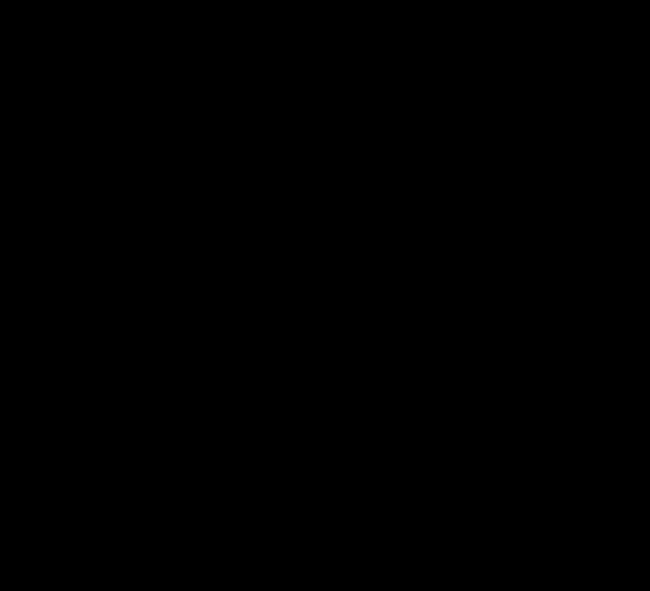
\includegraphics{toc-image}
  \medskip
  \caption*{ToC Entry}
\end{figure}

\end{document}
